\chapter{A NOVEL STIMLUI-RESPONSIVE HYDROGEL RECIPE FOR SOFT ROBOTICS: SYNTHESIS AND CHARACTERIZATION}
\label{chap:synthesis}
The ability to select from a broad range of material properties for SVA fabrication can expand the design space of resulting heterogeneous structures. Therefore, a synthesis method that can tune the ratio and rate of hydrogel volume change is required. 

We take advantage of PNIPAAm's cononsolvency, a property of reduced solvation in a mixture of two solvents due to a delicate balance between polymer-solvent and solvent-solvent interactions~\cite{Pica2016}. Employing a water and dimethyl sulfoxide (DMSO) mixed solvent in the PNIPAAm hydrogel precursor solution, followed by rapid photopolymerization to induce interconnected open pores, significantly enhanced the rate of water transport into and out of the hydrogel matrix and thus the actuation speed. The microstructure of the gel is altered by changing the water volume fraction (\(\varphi_{w}\)) in the mixed water/DMSO solvent. The SVA swelling rate and displacement, which are directly related to its hydrogel microstructure, are therefore tuned by merely  adjusting \(\varphi_{w}\). Polymerization solvent composition is known to affect the swelling properties of the synthesized PNIPAAm hydrogels~\cite{Wang2017e,Lee2000, Zhang2002a,Feng2011,Tokuyama2008}. 
%Rapid actuation using hydrogels requires ultrafast swelling speeds; 
The combination of the mixed solvent method with a fast 15\,s photopolymerization step is critical for inducing and fixing local aggregations of polymer chains in place,
% \rk{aggregation of polymer chains(what does it mean)}
resulting in PNIPAAm hydrogels with open pore structures (\firstsubfigref{fig:2}{A(i)}). Such open pore structures exhibit significantly enhanced rates of thermoresponsive volume change in both heating and cooling phases, compared to conventional hours-long mixed solvent thermopolymerization methods (control experiment), in which the precursors are constantly diffusing towards a homogeneous molecular equilibrium throughout the duration of the reaction, leading to a less interconnected pore structure with thicker pore walls (\subfigref{fig:2}{A(ii)}).
In order to ensure a valid comparison, the recipe for a representative thermopolymerized control hydrogel was carefully tuned using the initiator concentration while leaving all other components of the precursor solution unchanged, choosing a reaction time such that the conversion and water content match those of the photopolymerized hydrogel (Supporting Information and Table S2). It is readily observed that with equivalent water content, reaction conversion, and reaction solvent composition, the thermopolymerized hydrogel deswells as fast as the photopolymerized hydrogel \subfigref{fig:2}{B(i)} and the two reach nearly identical shrunken volumes (Figure S8, Supporting Information). However the reswelling speed of the thermopolymerized control sample is $\sim$25 times slower than the photopolymerized sample, which can be attributed to the lower observable tortuosity present in the photopolymerized sample \subfigref{fig:2}{B(ii)}. The Young's Modulus of the thermopolymerized hydrogel is $\sim$10 times higher than that of the photopolymerized one (Figure S9, Supporting Information).

The effect of varying \(\varphi_{w}\) on the hydrogel microstructure has been investigated by scanning electron microscopy (SEM), as shown in \subfigref{fig:2}{C}. Six hydrogels consisting of various \(\varphi_{w}\) were synthesized; they are each represented by a character code ranging from HG00 (representing a hydrogel with \(\varphi_{w}\) = 0.0) to HG05 (representing a hydrogel with \(\varphi_{w}\) = 0.5). Details of the SEM imaging procedure are described in the Supporting Information. Distinct changes in the microstructure can be observed as a function of \(\varphi_{w}\), which impacts a variety of other material properties. When \(\varphi_{w}\) is increased from 0.0 to 0.2, pore size decreases and the pore wall surface begins to change from smooth to rough. We define \(\varphi_{w}\) = 0.2 as a critical water volume fraction, at which the microstructure of the gel starts to change from a closed-pore to an open-pore structure. SEM images for other values of \(\varphi_{w}\) are presented in Figure S4 in the Supporting Information.
\begin{figure}[t]
\centering
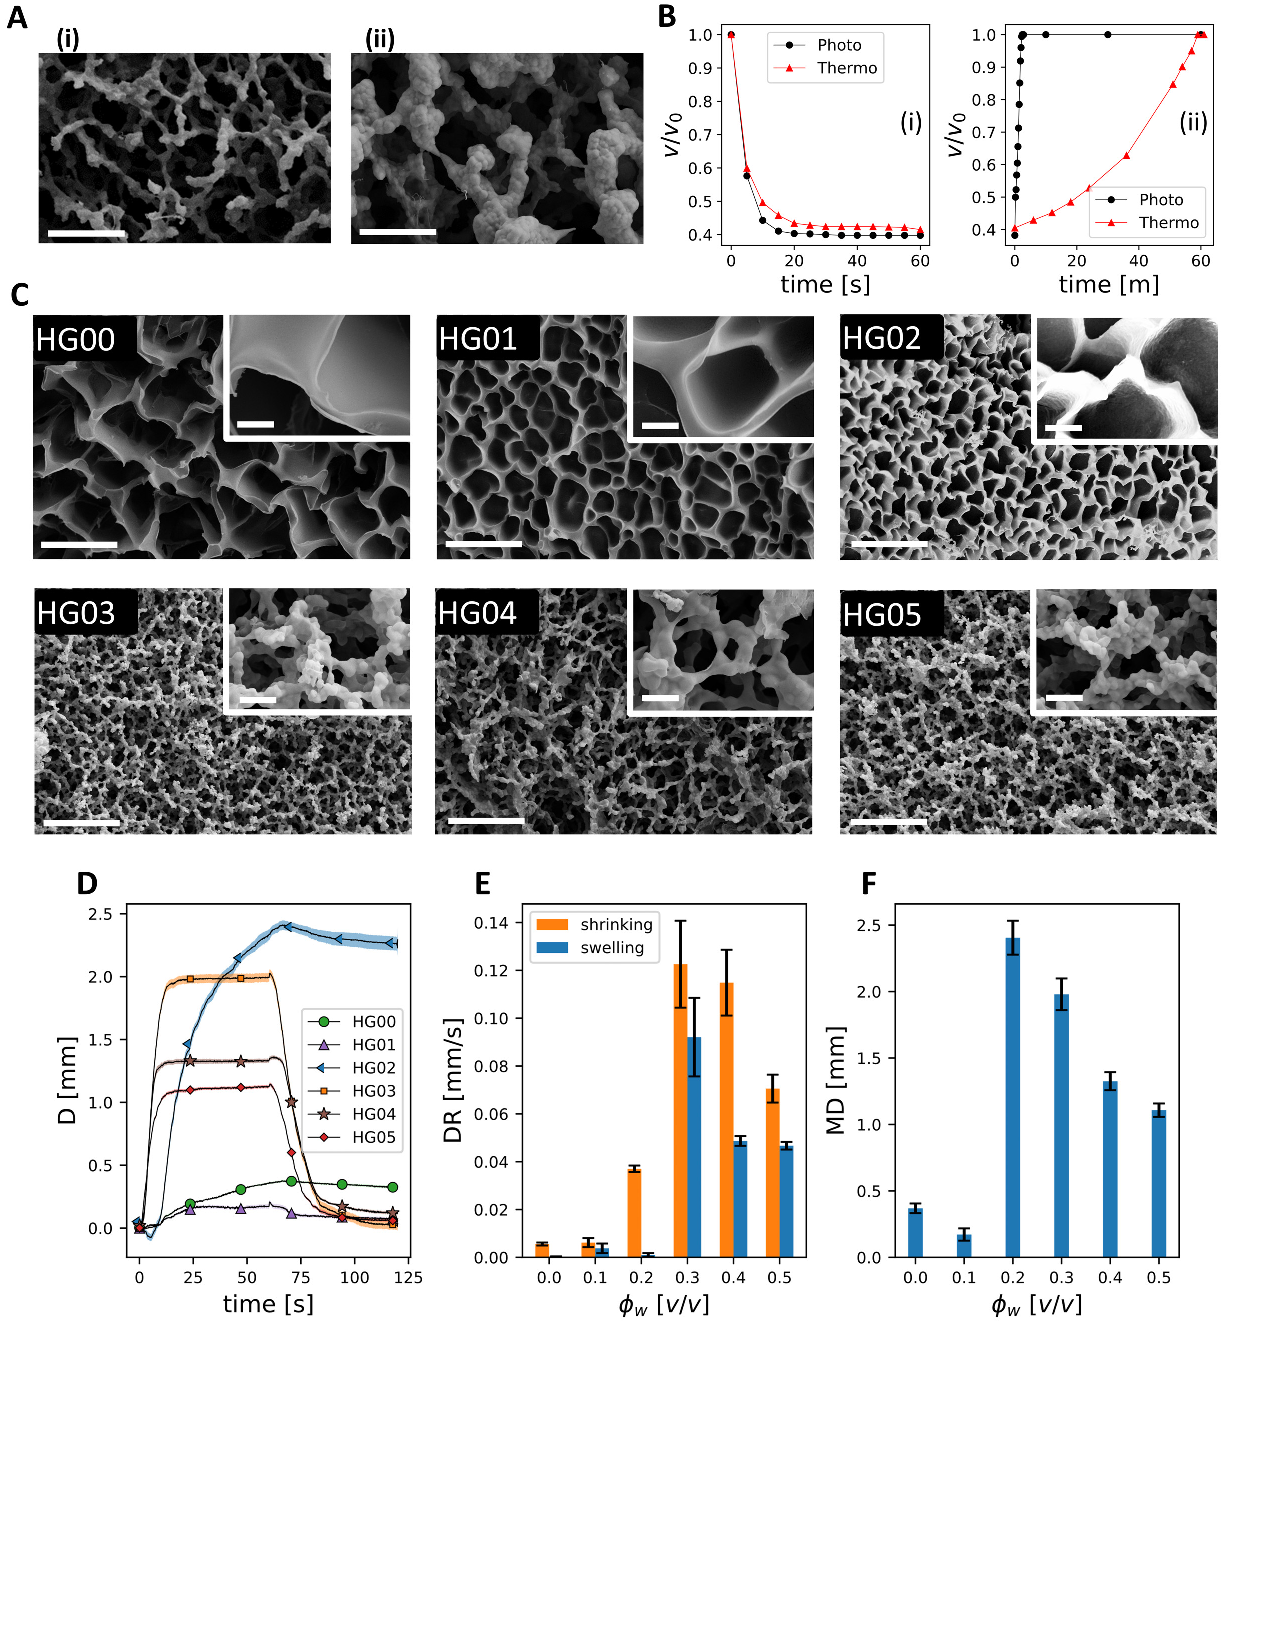
\includegraphics[width=0.9\textwidth]{Images/chap2/fig2.pdf}
\caption{Tunable material properties using mixed solvent photopolymerization.
% achieved by varying water volume fraction ($\varphi_w$) in the prepolymer mixture. 
\textbf{A)} SEM micrographs of photopolymerized (i) and thermopolymerized (ii) hydrogels synthesized in water volume fraction \(\varphi_{w}\)\,=\,0.27 (scale bar = $5\,\mu m$). \textbf{B)} Deswelling (i) and swelling (ii) rates of photopolymerized and thermopolymerized hydrogels synthesized in water volume fraction \(\varphi_{w}\)\,=\,0.27. \textbf{C)} SEM images showing the effect of $\varphi_w$ on pore structure of the photopolymerized PNIPAAm hydrogel (scale bars $10\,\mu m$ and $1\,\mu m$ for low and high magnification, respectively). \textbf{D)} Displacement (D) over time generated by SVA-II units with different values of \(\varphi_{w}\)  under a $1\,gf$ load, as measured by the setup described in the Supporting Information. \textbf{E,F)} Displacement rate (DR) and maximum displacement (MD) of SVA-II units as a function of $\varphi_w$,(extracted from B as described in the Supporting Information).}
% e) Compressive blocked force of a SVA-II f) Maximum compressive force as a function of $\varphi_w$ (extracted from e). 
% g) Young's modulus (E) as a function of SR. the data collection setup is described in methods.\note{change SR to $\varphi_w$}}
\label{fig:2}
\end{figure}
% \rk{this section should be rewritten to account for the fact that we have characterized actuators and not the material}
The changes in hydrogel microstructure play a role in the dynamic response of SVAs. The linear displacement generated by a SVA unit
% defined as the volume of the fully swollen SVA to that of dry gel -- 
is measured using a vision-based test setup as described and shown in the Supporting Information and Figure S3. \subfigref{fig:2}{D} plots the time evolution of the displacement ($D$) of SVA units with different values of $\varphi_w$ 
%as a function of time -- 
as each SVA's embedded heater is turned on for 60\,s 
% \rk{should a space be inserted between the s 60?} \xh{typically yes, between the number and unit} 
and then turned off for 60\,s. The displacement over time of the hydrogel made with \(\varphi_{w}\) = 0.0 is included as the basis for comparison across all tests. The negative displacement observed is because the SVAs initially expand instead of contract as the heater is turned on which might be due to water slightly expanding and vaporizing. Two performance criteria for the SVA units, deformation rate ($DR$) and maximum displacement ($MD$), are extracted from the data in \subfigref{fig:2}{D} and are shown in \subfigref{fig:2}{E,F} respectively. During both heating and cooling, $DR$ is small for \(\varphi_{w} < 0.2\). At \(\varphi_{w} = 0.2\), the $DR$ during heating is more than 36 times the $DR$ during cooling. As a result, fast and large deformations are observed during the 60\,s of heating, and almost no deformation is observed during the 60\,s of cooling. 
Highest $DR$ (in both heating and cooling) occurs in gels with $\varphi_w = 0.3$, while $MD$ peaks at $\varphi_w = 0.2$ and decrease thereafter.
% \note{more, or faster? rate or total shrinkage? use quantitative DR, MD etc..} 
% as the heater is turned on. When the heater is turned off, however, the gel does not swell during the 60s duration of the experiment.
In addition to swelling properties, other mechanical properties such as Young's modulus and force produced by the SVAs can also be tuned by adjusting \(\varphi_{w}\) (Figure S5, Supporting Information).\\ 

Hydrogels expand and contract based on the diffusion of water into and out of their structure when the temperature is passed their critical transition temperature -- which is around 32\textsuperscript{o} C in case of PNIPAAm hydrogels. 
discuss different actuator technologies
\section{Stimuli-responsive Hydrogels}
Stimuli-responsive Hydrogels also known as smart hydrogels, have attracted great interest in many different fields, such as drug delivery~\cite{Annabi2014,Stuart2010}, microfluidics \cite{DEramo2018a,Goy2019}, and soft robotics \cite{Banerjee2018}, owing to their large and reversible volume changes in response to a broad range of stimuli without using any additional sensors and actuators. This feature helps reduce the size of devices made of smart hydrogels. 


However, the equipment needed to create variable stimuli such as structured light \cite{palagi2016structured} or magnetic field \cite{Kim2018} are still bulky.  
Temperature responsive hydrogels, by contrast, can be stimulated electrically using Joule heating \cite{yu2013electronically}. The electrical stimulation can be confined to small regions making it possible to create more precise motions~\cite{richter2009optoelectrothermic}. 

We have previously reported solving some of the challenges associated with temperature responsive poly(N-isopropylacrylamide) (PNIPAAm) based hydrogels such as their slow response and tuning their mechanical properties. We have also introduced blocks called soft voxel actuators (SVAs), which are electrically activated by Joule heaters \cite{khodambashi2021heterogeneous}. 
In this communication, we demonstrate how SVAs support the development of soft robots which are miniature and untethered --two key characteristics that are challenging to realize with pneumatic soft actuators. We introduce a miniature completely untethered robot for underwater applications which weighs only 20\,g including battery and electronics as shown in Fig.~\ref{fig:concept}. We also demonstrate the use of SVAs to build a miniature continuum manipulator with hyper-redundant DOFs as shown in Fig.~\ref{fig:treajectory}A. This manipulator is 10$\times$ 40 $\times$ 4.5\,mm$^3$ and has 16 actuators. 

material characterization
sem images
mechanisms behind response rate
detailed literature review
\section{Section1}
\section{Section2}